这个算法的基础是假设聚类中心周围有局部密度较低的近邻点, 并且它们与任何局部密度较高的点都有比较大的距离。对于每个数据点$i$, 我们计算两个量: 它的局部密度$\rho_i$和它与密度较高的点的距离$\sigma_i$, 这两个量都只取决于数据点之间的距离$d_{ij}$, 假设这个距离满足三角不等式, 则数据点$i$的局部密度$\rho_i$被定义为
\begin{equation}
    \rho_i=\sum_{j}\chi (d_{ij}-d_c)
    \label{equ:1}
\end{equation}
其中, 如果$x<0$, 则$\chi(x)=1$, 否则$\chi(x)=0$, 而$d_c$是截止距离。基本上可以说是$\rho_i$等价于以$d_c$为半径的邻域内点的数量。该算法只对不同点的$\rho_i$的相对大小敏感, 这意味着, 对于大数据集, 其结果对$d_c$的选择是稳健的。

$\sigma_i$是通过计算点$i$和任何其他密度较高的点之间的最小距离来测量的: 
\begin{equation}
\delta_{i}=\min _{j: \rho_{j}>\rho_{i}}\left(d_{i j}\right)
\label{equ:2}
\end{equation}

对于密度最高的点, 习惯上取$\sigma_i = \max_j(d_{ij})$。需要注意的是只有对于密度为局部或全局最大值的点, $\sigma_i$才会比典型的最近邻距离大得多。因此, 聚类中心被认为是$\sigma_i$异常的点。
\begin{figure}[ht]
    \centering
    \subfigure[数据点的分布, 按密度递减的顺序排列。\label{fig:1a}]{
        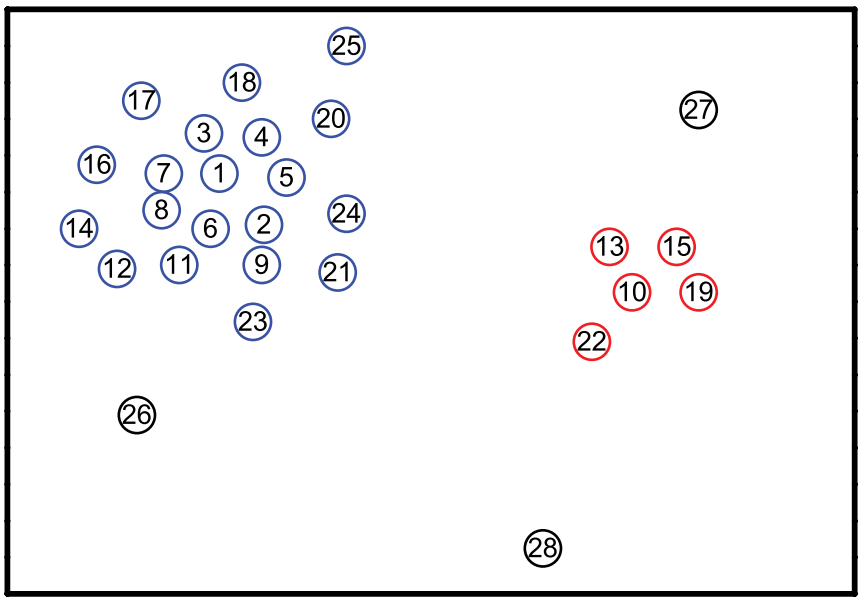
\includegraphics[scale=.21]{1_a.png}
    }
    \subfigure[(\ref{sub@fig:1a})中数据点的决策图, 不同的颜色对应不同的簇。\label{fig:1b}]{
        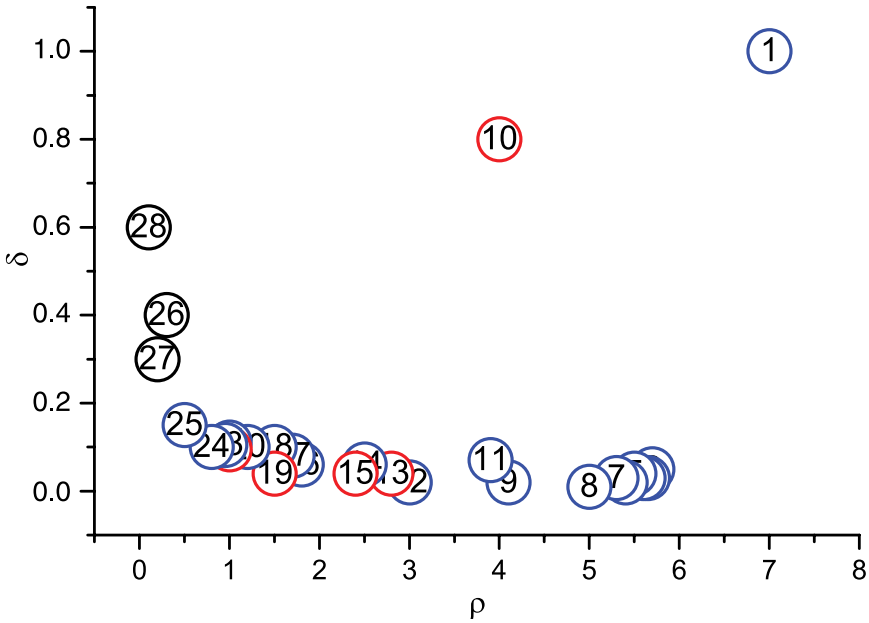
\includegraphics[scale=.20]{1_b.png}
    }
    \caption{算法在二维数据上的示例。\label{fig:1}}
\end{figure}

捕捉这个突变, 是算法的核心步骤, 图~\ref{fig:1}~中的简单例子就可以说明, 图~\ref{fig:1a}~是在二维空间中的28个点, 我们发现密度最大的点为1和10, 将其确定为聚类中心。图~\ref{fig:1b}~是每个点的$\sigma_i$与$\rho_i$的关系图, 我们将把它称为决策图。可以看到点9和10有相近的$\rho$值, 但却有差距很大的$\sigma$值, 而点9属于点1的簇, 其他几个$\rho$值较大的点离它很近, 而密度较高的点10属于另一个簇。因此, 只有具有较高$\sigma$和相对较高的$\rho$的点才是聚类中心。26、27、28点的$\sigma$较高, 但$\rho$相对较低, 因为它们基本上是孤立的, 因此可以认为它们是由单个点组成的簇, 即离群点。

在确定聚类中心后, 其余的点都会被分配到离其最近的簇中。与其他聚类算法不同的是, 此处的聚类分配是一步完成的, 其目标函数是迭代优化的\cite{MacQueen1967,McLachlan2007}。
\begin{figure}[ht]
    \centering
    \subfigure[数据的概率分布图示, 强度最低的区域对应$20\%$的概率。\label{fig:2a}]{
        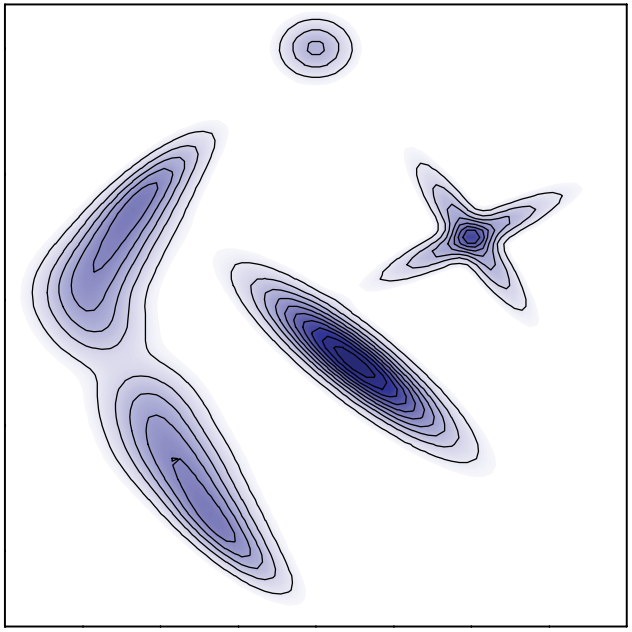
\includegraphics[scale=.20]{2_a.png}
    }\ 
    \subfigure[样本量为4000的数据分布结果, 黑色为噪声。\label{fig:2b}]{
        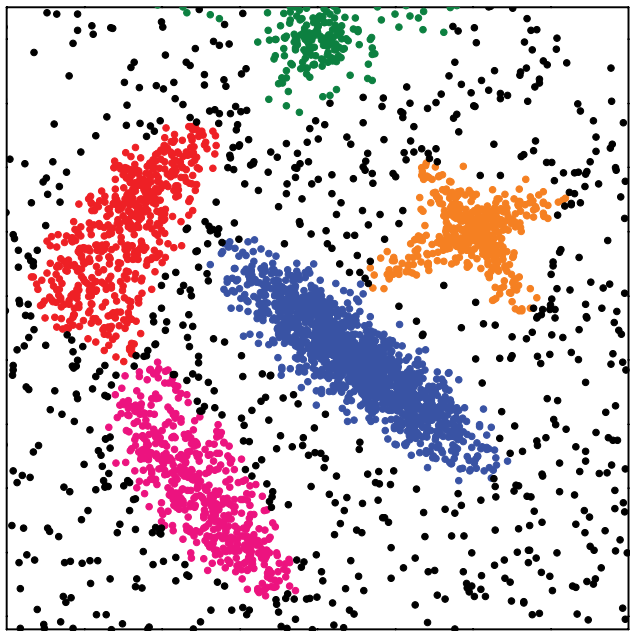
\includegraphics[scale=.20]{2_b.png}
    }\ 
    \subfigure[样本量为1000的数据分布结果, 黑色为噪声。\label{fig:2c}]{
        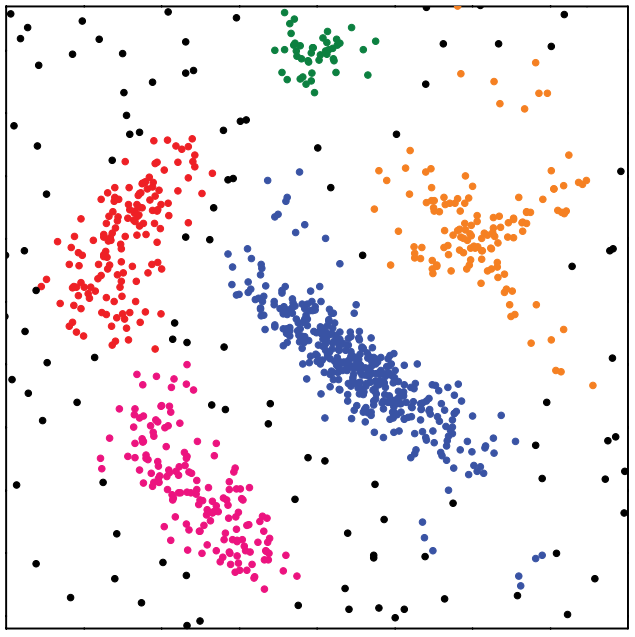
\includegraphics[scale=.20]{2_c.png}
    }\\
    \subfigure[样本量为4000的数据的决策图。\label{fig:2d}]{
        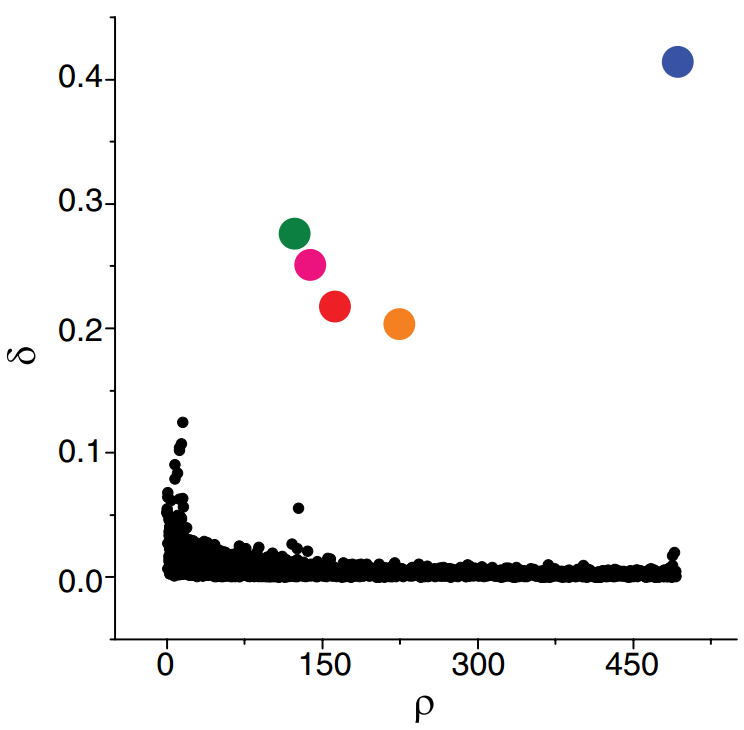
\includegraphics[scale=.18]{2_d.png}
    }\ 
    \subfigure[样本量为1000的数据的决策图。\label{fig:2e}]{
        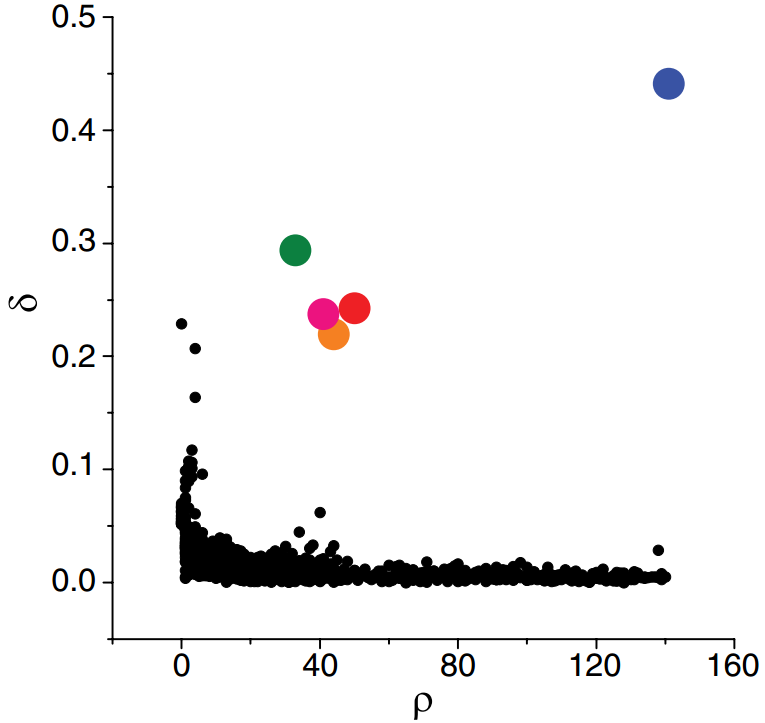
\includegraphics[scale=.18]{2_e.png}
    }\ 
    \subfigure[样本量和误分率的关系图, 误差条表示平均值的标准误差。\label{fig:2f}]{
        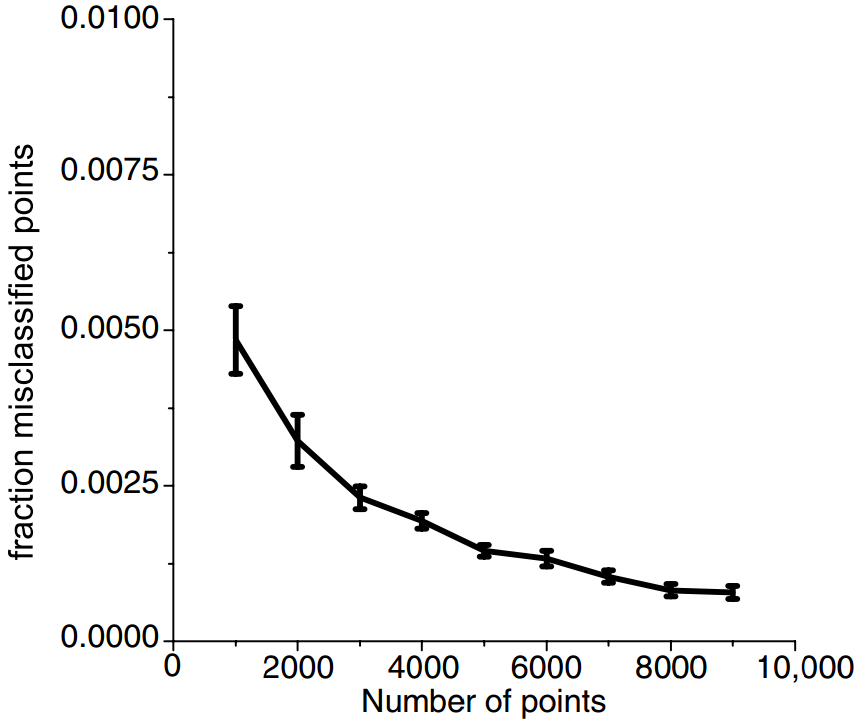
\includegraphics[scale=.18]{2_f.png}
    }
    \caption{算法在人工合成数据集上的示例。\label{fig:2}}
\end{figure}

在聚类分析中, 定量地衡量数据点的分配的可靠性往往是十分有用的, 在基于函数优化的方法中\cite{MacQueen1967,McLachlan2007}, 其收敛时的值也是对于可靠性的一种自然度量。在像DBSCAN\cite{Ester1996}这样的方法中, 人们会认为密度值高于某一阈值的点是可靠的, 这可能会导致低密度的聚类中心都被归为噪声, 如图~\ref{fig:2e}~所示。在我们的算法中, 我们并没有引入噪声信号的截止值, 相反, 我们首先为每个聚类找到一个边界区域, 定义为属于该类但与属于其他类的点的距离小于$d_c$的点的全体, 然后, 我们找出边界区域内密度最高的点, 用$\rho_b$表示其密度, 簇中密度高于$\rho_b$的点被认为是簇核的一部分(稳健分配), 其他的点被认为是簇环的一部分(可以被认为是噪声)。
